\section{Lineare Regression}
Lineare Regression ist eine einfache Methode um Daten zu analysieren.\\
Man nutzt es hauptsächlich für:
\begin{itemize}
\item \textbf{Interpretation}: Verstehen ob ein bestimmter Input ein Effekt hatfür den Output. Bsp: Gibt es eine Beziehung zwischen Raucher undLungenkrebs?
\item \textbf{Prediction}: Voraussehen wann was in Zukunft passieren könnte.Z.B. Wann geht eine Maschine kaputt anhand von Sensoren für Öldruck und Temperaturen
\end{itemize}
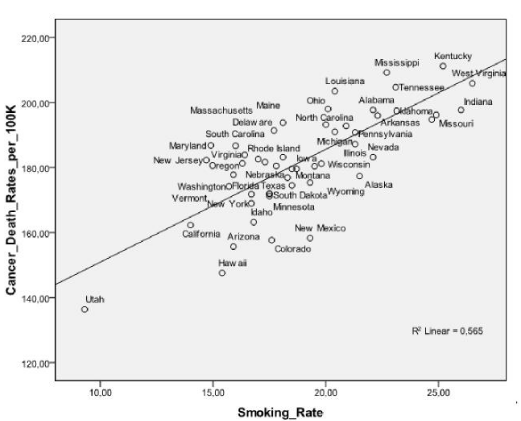
\includegraphics[width=\linewidth]{img/linear_regression.png}
\subsection{Linear Regression und Machine Learning}
Lineare Regression wird von Statistik «ausgeliehen». Hier ist es ein Beispiel von Algorithmen oder Techniken aus dem supervised learning. Wir haben also Inputdaten X und die Labels (In unserem Fall Y). Dann wird ein einfacher Algorithmus verwendet um daraus den Linearen Zusammenhang zu sehen. Das Modell soll also lernen Y vorauszusagen.\\
\\
\textcolor{myblue}{Model}\\
In ML Model steht für irgendeine mathematische Funktion, welche die Daten erklärt.
$$y_i \approx f(x_i)$$
$$y_i = f(x_i) + \epsilon_i$$

Das $\epsilon_i$ steht für «unerklärtes Rauschen». Man nimmt an, dass die der normalen Distribution folgt.\\
Die Funktion f kann beliebig kompliziert sein (Konstante oder Multi-Millionen-Parameter-Netzwerk). Machine Learning muss das korrekte Modell finden, welche die Daten möglichst gut interpretiert. Anstelle die Funktion näherungsweise zu bestimmen, bestimmen wir ein y-Hut, welche eine Schätzfunktion von $y_i$ ist.
$$y^\wedge_{i} = f(x_i)$$
In der Linearen Regression wird nur die Lineare Represäntation angeschaut zwischen input und output. Vor dem Lernen vom Algorithmus bestimmen wir den Model-Space (Funktionenschar). In einfachsten Fall sind x und y skalar und wir haben nur zwei frei wählbare, unbekannte Variablen a und b. Diese müssen wir nun mit Machine Learning bestimmen um möglichst nah an den Daten zu sein.
$$y^\wedge_{i} = a * x_i + b$$
a wird meist \textbf{slope} genannt und b \textbf{intercept}.\\
\textcolor{myblue}{Mean squared Error MSE (Loss, Residuals)}\\
Dies ist das \textbf{Loss} das wir minimieren wollen. (Hinweis: MSE ist normalerweise mit 2 dividiert)
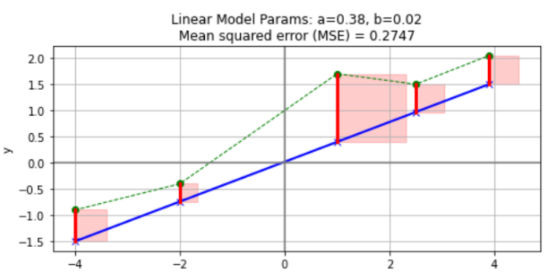
\includegraphics[width=\linewidth]{img/mse.png}
$$y^\wedge_{i} = a * x_i + b$$
$$e_i=y_i-y^\wedge_{i}$$
$$E=\frac{1}{2N}\sum_{i=1}^N e^2_i$$
$$=\frac{1}{2N}\sum_{i=1}^N(y_i-(a * x_i + b))^2$$
\subsection{Korrelation und Kausalität}
Korrelation ist \textbf{nicht} Kausalität!\\
Auch wenn der Koeffizient 0 ist können die Daten strukuriert sein -> Keine Aussagen über Kausalität machen. Immer Daten visualisieren und ebenso die Residuals.
\subsection{Komplexere Lineare Modelle}
EVTL TODO
\subsection{Uniform Distrubution, Normal Distribution}
Evtl TODO: Übernehmen aus ExEv Howtosolve
\subsection{Seaborn Jointplot}
Der Jointplot ist eine Verbindung von zwei Variablen mit bivariaten und univariaten Graphen. Es zeigt die (empirischen) Randverteilungen als Histogramme. Das Ergebnis ist ideal: die Daten (x-Werte) sind gleichmäßig über den gesamten Bereich verteilt (Gleichverteilung in -50/+50), während die Residuen bei 0 zentriert sind (Standardnormalverteilung).
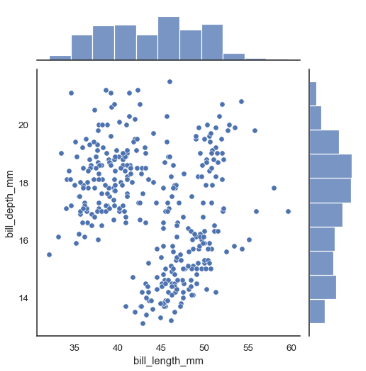
\includegraphics[width=\linewidth]{img/seaborn_jointplot.png}